% =============================================================================
% BudgetBench: Budget-Constrained Evaluation Harness for Tool-Using Code Agents
% CMU 24-880 AI Agents for Engineers — Spring 2026 Final Report
% Team 14: Chenrui Xu, Hanyu Jin, Sylvia Li
% =============================================================================
%
% NOTE on template:
%   Canvas template was not provided. This file uses a clean single-column
%   article style targeting 6–8 pages. If a Canvas template is required,
%   copy the body sections (after \maketitle) into that template's main file.
% =============================================================================

\documentclass[11pt]{article}

\usepackage[margin=1in]{geometry}
\usepackage[utf8]{inputenc}
\usepackage{amsmath,amssymb,amsthm}
\usepackage{graphicx}
\usepackage{booktabs}
\usepackage{xcolor}
\usepackage{hyperref}
\usepackage{url}
\usepackage{microtype}
\usepackage{caption}
\usepackage{subcaption}
\usepackage{listings}
\usepackage{authblk}

\hypersetup{colorlinks=true, linkcolor=blue!50!black, citecolor=blue!50!black,
            urlcolor=blue!50!black}

\graphicspath{
  {../results/figures/}
  {../results/final/}
  {../results/knapsack_pro/}
  {../results/swe_5issues_flash/}
  {figures/}
}

\lstset{
  basicstyle=\ttfamily\footnotesize,
  breaklines=true,
  showstringspaces=false,
  columns=fullflexible,
  frame=single,
  framesep=3pt,
}

\title{\textbf{BudgetBench: A Budget-Constrained Evaluation Harness for Tool-Using Code Agents}}

\author[1]{Chenrui Xu}
\author[1]{Hanyu Jin}
\author[1]{Sylvia Li}
\affil[1]{Carnegie Mellon University \\ \texttt{\{chenrui2, hanyuj, yangli6\}@andrew.cmu.edu}}
\date{April 28, 2026}

\begin{document}
\maketitle

% -----------------------------------------------------------------------------
\begin{abstract}
Existing code-agent benchmarks rank agents by terminal correctness and ignore
how many tool calls were spent reaching that answer. Two agents that solve
the same issue, one in 5 calls and one in 50, receive identical scores even
though their deployment costs differ by an order of magnitude. We introduce
\textbf{BudgetBench}, an evaluation harness that makes the tool-call budget
a first-class axis. The framework intercepts every action an agent takes,
tracks cumulative cost against a configured ceiling, and reports
Success@B, the AUC of the success-versus-budget curve, and the budget
violation rate, with bootstrap confidence intervals. We instantiate the
harness on two environments (a deterministic Knapsack toy environment and
SWE-bench Lite) and study three agents: a single-shot baseline, a standard
ReAct-style loop, and a regime-switching \emph{BudgetAwareAgent} that adapts
its strategy as remaining budget shrinks. Across 900 Knapsack episodes and 96 SWE-bench Lite episodes
(8 issues, 3 agents, 2 budgets, 2 Gemini variants), the
budget-aware agent matches the
single-shot agent's terminal success while keeping the budget violation
rate at zero, whereas the unmodified loop agent collapses at low budgets
regardless of which Gemini model backs it. Upgrading from Gemini 2.5
Flash to Pro adds a uniform 8 percentage points across all agents but does
not change the qualitative ordering, suggesting that under tight budgets
agent design dominates model capability.
\end{abstract}

% -----------------------------------------------------------------------------
\section{Introduction}
\label{sec:intro}

Modern code-agent benchmarks ask a simple question: does the agent produce
a patch that resolves the target issue? SWE-bench~\cite{jimenez2024swebench} and
its variants score every successful patch identically, regardless of how
much computation the agent spent finding it. Yet practitioners deploying
these agents care intensely about cost. A coding agent that uses 5 tool
calls to fix a bug at \$0.01 dominates one that needs 50 calls at \$0.50,
even though both score 1.0 on standard leaderboards. The benchmark cannot
see the difference; the engineering team cannot ignore it.

The gap between scoring and deployment is not just a units mismatch. It
distorts agent design. ReAct-style loops~\cite{yao2023react} are encouraged
to over-explore because each additional search, inspect, or test call
costs them nothing in the metric. Newer multi-step agents push the same
direction. The question \emph{can this agent solve the problem in time?}
has no formal place in the evaluation, so it gets answered by accident
or by hand-tuning. \emph{Pass@k}~\cite{chen2021codex} measures sample
efficiency at the level of complete attempts but says nothing about the
action efficiency \emph{within} an attempt.

This paper contributes (1) \textbf{BudgetBench}, a small harness that
exposes a per-episode tool-call budget as a first-class axis and emits
the metrics needed to study how agents behave as the budget tightens;
(2) two reference environments at very different scales, namely a
deterministic 0/1-knapsack environment for harness validation and
SWE-bench Lite for realistic patching; (3) three reference agents
including a regime-switching \textbf{BudgetAwareAgent} that adapts its
strategy as remaining budget shrinks; and (4) an empirical study
spanning 900 Knapsack episodes plus 96 SWE-bench Lite episodes,
including a Gemini 2.5 Flash versus Pro comparison on both
environments.

Our main finding is that, in the budget-constrained regime, a small
amount of strategy beats a large amount of model. The BudgetAwareAgent
matches the single-shot baseline's terminal accuracy at every budget
level we test while keeping its budget-violation rate at zero. The
unmodified ReAct-style loop collapses at low budgets, exhausting its
allotment before submitting any patch, and switching its backbone from
Gemini Flash to Pro raises its score by only a few percentage points
without changing the qualitative picture. The cost of adding budget
awareness was roughly one hundred lines of Python.

% -----------------------------------------------------------------------------
\section{Related Work}
\label{sec:related}

\paragraph{Code-agent benchmarks.}
SWE-bench~\cite{jimenez2024swebench} and its lighter sibling SWE-bench
Lite~\cite{swebenchlite2024} have become the standard for evaluating
end-to-end issue resolution in real Python repositories. Both judge an
agent solely by whether the submitted patch passes the hidden test suite.
Earlier function-level benchmarks such as HumanEval~\cite{chen2021codex}
and MBPP~\cite{austin2021mbpp} are similarly silent on the cost of producing
each solution.

\paragraph{Tool-using agents.}
ReAct~\cite{yao2023react} introduced the now-standard interleaving of
reasoning and tool calls, and Toolformer~\cite{schick2023toolformer} explored
self-supervised tool acquisition. Recent SWE-bench-targeted systems such
as SWE-Agent~\cite{yang2024sweagent} extend the paradigm with dedicated
agent-computer interfaces. None of these works expose a tool-call budget
as a first-class evaluation parameter, although several mention that
practical deployments cap the number of steps for cost reasons.

\paragraph{Cost-aware evaluation.}
Pass@k~\cite{chen2021codex} captures sample efficiency across independent
attempts. HELM~\cite{liang2023helm} reports per-query token and dollar cost
alongside accuracy, but treats cost as a post-hoc audit rather than a
per-episode constraint. Our work differs by enforcing the budget
\emph{during} an episode and measuring how performance degrades as the
ceiling is lowered.

\paragraph{Anytime and budget-aware planning.}
Anytime algorithms~\cite{zilberstein1996anytime} have studied
quality-versus-deliberation-time trade-offs since the 1990s.
BudgetBench provides the infrastructure to measure such trade-offs in
modern LLM agents rather than demonstrate any particular adaptation
mechanism.


% -----------------------------------------------------------------------------
\section{The BudgetBench Framework}
\label{sec:framework}

\subsection{Core Abstractions}
\label{sec:framework:abstractions}

BudgetBench is built around four lightweight abstractions. An
\texttt{Agent} exposes a single method
\texttt{act(obs, budget\_remaining, history) $\rightarrow$ ToolCall},
which returns the next tool call to execute. An \texttt{Environment} is
the world the agent acts in: it accepts a tool call, returns an
\texttt{Observation}, and provides a final scoring hook that decides
whether a submitted patch resolves the underlying task. A
\texttt{BudgetRunner} glues the two together, intercepts every tool call
issued by the agent, debits its cost from a configured budget, and
terminates the episode the moment the running total exceeds the ceiling.
Each run produces an immutable \texttt{Episode} object containing the
full trace and one of four terminal statuses: \texttt{OK\_SOLVED},
\texttt{TEST\_FAIL}, \texttt{INVALID\_FORMAT}, or
\texttt{BUDGET\_EXCEEDED}. These four status codes form the basis of
every metric in the next section.

The contract is deliberately minimal. An agent that already targets
SWE-bench typically needs only a thin shim to expose its existing tool
loop as \texttt{act}, after which it gains budget enforcement,
deterministic logging, and metric reporting at no additional cost. The
runner itself is roughly two hundred lines of Python and has no
LLM-specific dependencies.

\begin{figure}[t]
  \centering
  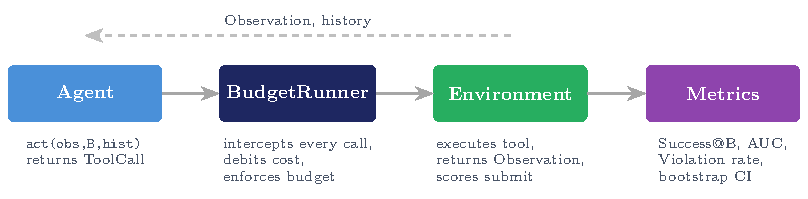
\includegraphics[width=0.95\textwidth]{architecture.pdf}
  \caption{BudgetBench architecture. The BudgetRunner intercepts every tool
  call from the agent, tracks cumulative cost against the configured budget,
  and terminates the episode the moment the budget is exhausted.}
  \label{fig:architecture}
\end{figure}

\subsection{Cost Model}
\label{sec:framework:cost}

Not every tool call is equally expensive in practice, and the cost model
should reflect this. By default each lightweight call (\texttt{search},
\texttt{inspect}, \texttt{edit}, \texttt{hierarchy}, and the knapsack
manipulation tools) debits one unit of budget. Running the issue's test
suite costs three, reflecting that real-world test runs can take seconds
or minutes and dominate the wall-clock and dollar cost of a full episode
when invoked repeatedly. Submitting the final patch costs zero, since by
the time \texttt{submit\_patch} is called the agent has committed to its
answer and any further work is wasted. Table~\ref{tab:cost} lists the
defaults; cost weights are configurable per experiment.

\begin{table}[t]
  \centering
  \caption{Default tool cost weights.}
  \label{tab:cost}
  \begin{tabular}{lr}
    \toprule
    Tool & Cost \\
    \midrule
    \texttt{search}, \texttt{inspect}, \texttt{hierarchy}, \texttt{edit} & 1 \\
    \texttt{list\_items}, \texttt{add\_item}, \texttt{remove\_item}, \texttt{check\_feasibility} & 1 \\
    \texttt{run\_tests} & 3 \\
    \texttt{submit\_patch} & 0 \\
    \bottomrule
  \end{tabular}
\end{table}

\subsection{Metrics}
\label{sec:framework:metrics}

For an agent run on $N$ episodes with terminal statuses $s_1, \ldots, s_N$
and budget usage $b_1, \ldots, b_N$, we report four quantities. Let
$\mathbb{1}[\cdot]$ denote the indicator function.
\begin{align*}
\text{Success@B}    &= \tfrac{1}{N} \sum_i \mathbb{1}[s_i = \text{OK\_SOLVED} \land b_i \le B] \\
\text{Invalid@B}    &= \tfrac{1}{N} \sum_i \mathbb{1}[s_i = \text{INVALID\_FORMAT}] \\
\text{Violation@B}  &= \tfrac{1}{N} \sum_i \mathbb{1}[s_i = \text{BUDGET\_EXCEEDED}] \\
\text{AUC}          &= \tfrac{1}{B_\text{max}} \int_{0}^{B_\text{max}} \text{Success@B} \, dB
\end{align*}
The integral is approximated by the trapezoidal rule over the tested
budget grid. We accompany Success@B with a 95\% bootstrap confidence
interval using 1000 resamples over the per-episode outcomes. As a
secondary diagnostic we also report Time-to-First-Valid (TTFV), the
mean budget consumed before the agent first issues a syntactically
valid \texttt{submit\_patch}, which captures how quickly an agent
commits to an answer regardless of correctness.

We treat AUC as the primary ranking metric because it rewards agents
that succeed across the whole budget range rather than only at
$B_\text{max}$. An agent that achieves 60\% success at every budget
dominates an agent that achieves 80\% only at the maximum budget but
nothing below. Success@$B_\text{max}$ alone hides this gap; AUC exposes
it.

% -----------------------------------------------------------------------------
\section{Environments}
\label{sec:envs}

\subsection{Knapsack (Toy)}
\label{sec:envs:knapsack}

The Knapsack environment instantiates the classic 0/1 knapsack problem
inside the BudgetBench interface. Each episode generates ten items with
weights and values drawn uniformly from $[1, 20]$ given a fixed seed,
and the agent must select a subset that fits the capacity 50 while
maximising total value. The agent interacts through five tools:
\texttt{list\_items} returns the candidate set; \texttt{add\_item} and
\texttt{remove\_item} mutate the current selection;
\texttt{check\_feasibility} reports whether the current selection
respects capacity and what items are in it; \texttt{submit\_patch}
finalises the answer. A dynamic-programming oracle scores each submission
against the optimal value, returning \texttt{OK\_SOLVED} only on an exact
match.

We use Knapsack purely as a harness shakedown. It is fully deterministic
given a seed, requires no API key, runs in milliseconds, and isolates
agent strategy from LLM stochasticity. The fifty seeds we use are reused
identically across every (agent, budget, model) cell, so any difference
in outcomes is attributable to those three axes alone. The Knapsack
agents in our reported experiments are heuristic, not LLM-backed; this
choice keeps the comparison cheap to reproduce and removes the
confounder of prompting differences.

\subsection{SWE-bench Lite}
\label{sec:envs:swe}

SWE-bench Lite~\cite{swebenchlite2024} is a curated subset of
SWE-bench~\cite{jimenez2024swebench} consisting of real GitHub issues from
popular Python repositories together with their hidden test suites.
Our wrapper loads the dataset, starts a Docker container per episode
from the official SWE-bench evaluation image (which has the repository
pre-installed at the issue's base commit), and exposes six tools:
\texttt{search} runs a grep-style query across the repository,
\texttt{inspect} reads file lines, \texttt{hierarchy} prints the
directory tree, \texttt{edit} applies a unified diff to a single file,
\texttt{run\_tests} executes the issue's test suite inside the sandbox,
and \texttt{submit\_patch} finalises the agent's diff for scoring.

Scoring follows a two-tier strategy. We first attempt the official
SWE-bench harness via \texttt{python -m swebench.harness.run\_evaluation}
and read the resulting summary JSON. If the issue identifier appears
under \texttt{resolved\_ids} the patch is recorded as
\texttt{OK\_SOLVED}; if it appears under \texttt{error\_ids} we fall
through to a manual fallback that re-applies the patch in a fresh
sandbox, runs the issue's \texttt{PASS\_TO\_PASS} and
\texttt{FAIL\_TO\_PASS} test sets directly, and reports the corresponding
status. Falling through rather than instantly failing is important: in
practice the harness reports errors for several recoverable conditions
(image-tag mismatches, transient Docker failures) where a simple manual
re-run still yields a clean answer.

For this study we use eight default-ordering Lite issues spanning
\texttt{astropy} (four issues) and \texttt{django} (four issues). We dropped two
further astropy issues because their official evaluation images
required an environment image variant we could not pre-cache in time. The \texttt{run\_tests} cost is set to three (versus one for all
other tools) reflecting the wall-clock and resource cost of actually
running a real test suite.

% -----------------------------------------------------------------------------
\section{Agents}
\label{sec:agents}

\subsection{SingleShotAgent}
\label{sec:agents:singleshot}

SingleShotAgent issues exactly one LLM call. It reads the issue
description, produces a unified diff, and calls \texttt{submit\_patch}
immediately. Its budget consumption is therefore independent of the
budget ceiling: the only call it ever makes is \texttt{submit\_patch},
which costs zero. This makes it a natural lower-effort baseline that
isolates raw model capability from any agentic strategy. Any agent that
fails to beat SingleShot at a given budget is failing to put its
exploration tools to good use.

\subsection{LoopAgent}
\label{sec:agents:loop}

LoopAgent implements the standard ReAct-style tool loop. At each step
it sends the issue description, the recent action and observation
history, and the available tool list to a Gemini chat session, then
parses the model's response into a single tool call. The cycle repeats
until the agent voluntarily issues \texttt{submit\_patch} or the runner
terminates the episode for exceeding budget. Crucially, the prompt does
not include the remaining budget, and the agent has no mechanism for
adapting its behaviour as the ceiling approaches. This is the
implementation choice we expect to expose: an agent that explores until
it is satisfied, regardless of cost, is exactly the design that
unrestricted benchmarks reward.

\subsection{BudgetAwareAgent (key novelty)}
\label{sec:agents:budgetaware}

BudgetAwareAgent extends LoopAgent with a single idea: at every step,
look at the fraction of budget remaining and switch strategy
accordingly. We define three regimes by the remaining-budget fraction
$f = \texttt{budget\_remaining} / \texttt{budget\_total}$.

In the \emph{HIGH} regime ($f > 0.6$) the agent behaves exactly like
LoopAgent with the full toolset. In the \emph{MEDIUM} regime
($0.3 < f \le 0.6$) the agent prunes \texttt{run\_tests} from its
allowed actions; given that \texttt{run\_tests} costs three units, this
single change roughly triples the number of remaining exploratory
moves. In the \emph{LOW} regime ($f \le 0.3$) the agent stops calling
the LLM altogether, extracts the most recent valid diff from its
history, and submits it. The intuition is that once the budget is
nearly spent, more LLM thinking is unlikely to find a fundamentally
better patch and a cheap fallback dominates the alternative
(\texttt{BUDGET\_EXCEEDED}).

The implementation reuses the LoopAgent code path. We introduced a
shared \texttt{\_BaseLoopAgent} class containing the common chat-loop
machinery and overrode three hooks: \texttt{\_regime\_section()}
injects a short instruction block into the system prompt describing
the current regime, \texttt{\_pre\_act()} short-circuits the LLM call
in the LOW regime, and \texttt{\_allow\_run\_tests()} returns
\texttt{False} in MEDIUM. The new code is roughly 120 lines. Regime
thresholds (0.6 and 0.3) are hand-tuned and identical across all of
our experiments; learning them per environment is left for future
work.

\begin{figure}[t]
  \centering
  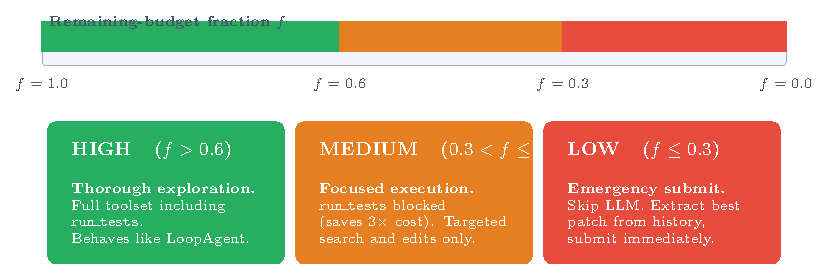
\includegraphics[width=0.95\textwidth]{regimes.pdf}
  \caption{BudgetAwareAgent's three regimes. The agent observes its remaining
  budget fraction $f$ at every step and switches strategy: HIGH explores freely,
  MEDIUM blocks the expensive \texttt{run\_tests} action, LOW skips the LLM
  call entirely and submits the best patch seen so far.}
  \label{fig:regimes}
\end{figure}

% -----------------------------------------------------------------------------
\section{Experiments}
\label{sec:exp}

\subsection{Setup}
\label{sec:exp:setup}

We launch all experiments through a single
\texttt{scripts/batch\_experiment.py} entry point that takes the
environment, agent set, model name, issue list, and budget list as
arguments. We fix random seeds per (environment, issue) so that every
(agent, budget, model) combination sees an identical task distribution. The Knapsack environment runs locally and uses heuristic
agents; the SWE-bench environment uses Gemini 2.5 Flash and Gemini 2.5
Pro for the LLM agents and the official SWE-bench evaluation Docker
images for the sandbox. Table~\ref{tab:design} summarises the cells we
report.

\begin{table}[t]
  \centering
  \caption{Experimental design.}
  \label{tab:design}
  \begin{tabular}{llrrr}
    \toprule
    Environment & Model & Issues / seeds & Budgets & Episodes \\
    \midrule
    Knapsack       & Flash    & 50 seeds       & 5, 10, 20    & 450 \\
    Knapsack       & Pro      & 50 seeds       & 5, 10, 20    & 450 \\
    SWE-bench Lite & Flash    & 8 issues       & 20, 40       & 48  \\
    SWE-bench Lite & Pro      & 8 issues       & 20, 40       & 48  \\
    \multicolumn{2}{l}{\textbf{Total}} &  &  & \textbf{996} \\
    \bottomrule
  \end{tabular}
\end{table}

\subsection{Knapsack Results}
\label{sec:exp:knapsack}

Three results stand out from Table~\ref{tab:knapsack} and
Figure~\ref{fig:knapsack-flash-pro}. First, SingleShot and BudgetAware
reach the same Success@B at every budget level we tested, namely 0.62
under Flash and 0.70 under Pro. The two agents converge because
BudgetAware's regime logic happens to fall back to the same greedy
heuristic SingleShot uses by default in the LOW regime; this is the
intended behaviour, not a coincidence. Second, LoopAgent collapses at
low budgets: it scores zero at $B \in \{5, 10\}$ and barely above
chance ($0.08$ Flash, $0.12$ Pro) at $B = 20$. All of its low-budget
failures are \texttt{BUDGET\_EXCEEDED}, meaning it never even submitted
a candidate. Third, the Flash-to-Pro improvement is a uniform 8 percentage
points across all agents and budgets, consistent with Pro being a
strictly stronger backbone that contributes nothing to budget discipline. BudgetAware's violation
rate is zero across its 150 Knapsack episodes per model (50 seeds
$\times$ 3 budgets); LoopAgent's violation rate is 100\% at $B \le 10$.

The Time-to-First-Valid (TTFV) column in Table~\ref{tab:knapsack}
explains the AUC gap mechanically. SingleShot submits at TTFV $= 1$
(one \texttt{list\_items} call followed by a free \texttt{submit\_patch}).
BudgetAware's TTFV scales linearly with budget at $0.4 \cdot B$
(2.0, 4.0, 8.0 at $B = 5, 10, 20$), which is exactly the budget it
spends in the HIGH regime before its 0.6 threshold tips it into the
fallback path. LoopAgent only ever produces a valid submit at $B = 20$,
and even then it consumes 17.9 of the 20 available units before doing
so. The success curve and the TTFV column together separate
``efficient'' from ``eventually correct'' agents.

\begin{figure}[t]
  \centering
  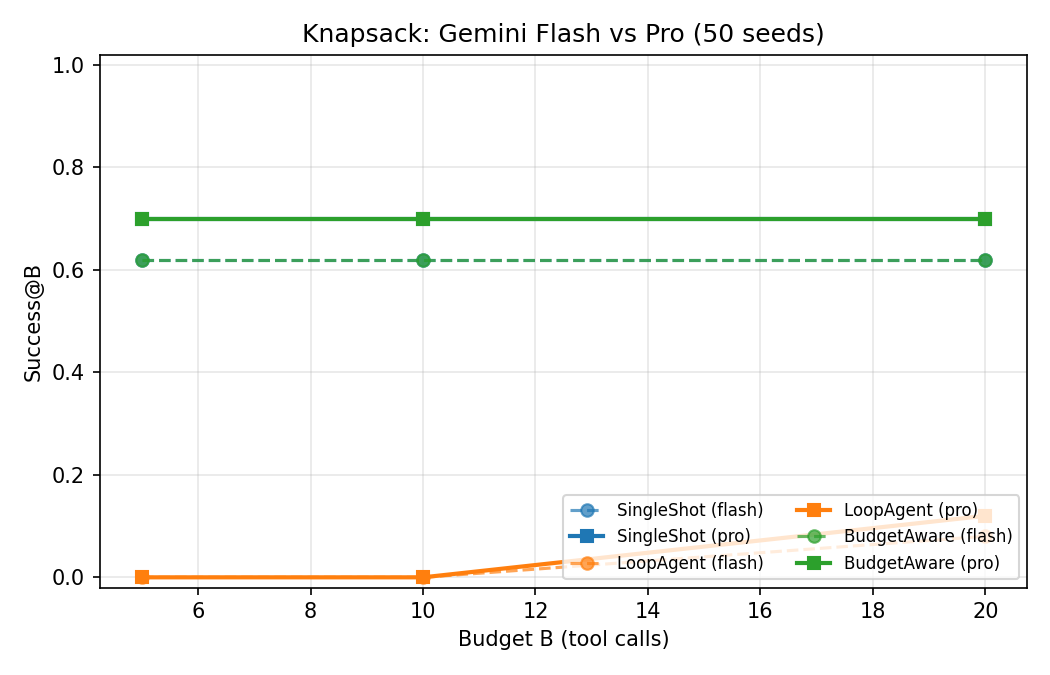
\includegraphics[width=0.8\textwidth]{knapsack_flash_vs_pro.png}
  \caption{Knapsack: Success@B for Flash (dashed) vs Pro (solid). Pro
  improves uniformly by $\sim$8 percentage points across all agents and
  budgets, but does not change the qualitative picture: LoopAgent collapses
  at low budgets regardless of model size.}
  \label{fig:knapsack-flash-pro}
\end{figure}

\begin{table}[t]
  \centering
  \caption{Knapsack: Success@B with 95\% bootstrap CIs (n=50 seeds per cell,
  1000 resamples), AUC of the success-versus-budget curve at $B_\text{max}=20$,
  and TTFV (mean budget consumed before the agent's first valid
  \texttt{submit\_patch}; ``--'' means the agent never submitted within budget).
  Pro dominates Flash by $\sim$8\,pp on Success@B; BudgetAware ties SingleShot
  on terminal success but spends roughly $0.4 \cdot B$ on exploration before
  falling back, which costs it AUC.}
  \label{tab:knapsack}
  \footnotesize
  \begin{tabular}{llcccccc}
    \toprule
    Agent & Model & Succ@5 & Succ@10 & Succ@20 & 95\% CI & AUC@20 & TTFV@20 \\
    \midrule
    SingleShot  & Flash & 0.62 & 0.62 & 0.62 & [0.48, 0.76] & 0.589 & 1.0 \\
    SingleShot  & Pro   & 0.70 & 0.70 & 0.70 & [0.56, 0.82] & 0.665 & 1.0 \\
    LoopAgent   & Flash & 0.00 & 0.00 & 0.08 & [0.02, 0.16] & 0.016 & 17.9 \\
    LoopAgent   & Pro   & 0.00 & 0.00 & 0.12 & [0.04, 0.22] & 0.019 & 17.9 \\
    BudgetAware & Flash & 0.62 & 0.62 & 0.62 & [0.48, 0.76] & 0.388 & 8.0 \\
    BudgetAware & Pro   & 0.70 & 0.70 & 0.70 & [0.56, 0.82] & 0.438 & 8.0 \\
    \bottomrule
  \end{tabular}
\end{table}

\subsection{SWE-bench Lite Results}
\label{sec:exp:swe}

SWE-bench Lite is a much harder environment than Knapsack and the
qualitative picture changes accordingly. Table~\ref{tab:swe} reports
Success@B for the eight-issue Flash run.

\begin{table}[t]
  \centering
  \caption{SWE-bench Lite (eight issues per cell). Success@B with 95\%
  bootstrap CIs, AUC, and budget-violation rate (Viol\%) for both
  Gemini 2.5 Flash and Pro. The strongest cell is BudgetAware @ Pro at
  $B{=}20$, which solves five of eight issues with zero violations.
  Switching to Pro eliminates LoopAgent's Flash budget violations
  entirely.}
  \label{tab:swe}
  \footnotesize
  \begin{tabular}{lllcccc}
    \toprule
    Agent & Model & B & Succ@B & 95\% CI & AUC & Viol\% \\
    \midrule
    SingleShot  & Flash & 20 & 0.000 & [0.00, 0.00] & 0.000 & 0\% \\
    SingleShot  & Flash & 40 & 0.000 & [0.00, 0.00] & 0.000 & 0\% \\
    SingleShot  & Pro   & 20 & 0.000 & [0.00, 0.00] & 0.000 & 0\% \\
    SingleShot  & Pro   & 40 & 0.000 & [0.00, 0.00] & 0.000 & 0\% \\
    LoopAgent   & Flash & 20 & 0.375 & [0.13, 0.75] & 0.091 & 38\% \\
    LoopAgent   & Flash & 40 & 0.375 & [0.13, 0.75] & 0.164 & 13\% \\
    LoopAgent   & Pro   & 20 & 0.375 & [0.00, 0.75] & 0.259 & 0\% \\
    LoopAgent   & Pro   & 40 & 0.500 & [0.13, 0.88] & 0.441 & 0\% \\
    BudgetAware & Flash & 20 & \textbf{0.625} & [0.25, 0.88] & 0.322 & 0\% \\
    BudgetAware & Flash & 40 & 0.375 & [0.00, 0.75] & 0.173 & 0\% \\
    BudgetAware & Pro   & 20 & \textbf{0.625} & [0.25, 0.88] & 0.378 & 0\% \\
    BudgetAware & Pro   & 40 & 0.500 & [0.13, 0.88] & \textbf{0.438} & 0\% \\
    \bottomrule
  \end{tabular}
\end{table}

Three observations stand out. First, SingleShot solves none of the 16
SWE-bench episodes. Without exploration, the model cannot guess a
patch that resolves any of the eight selected astropy and django
issues; every submission lands in \texttt{TEST\_FAIL}. This is the
expected outcome on a benchmark where issues require multi-file
reasoning and a strict test suite, and confirms that Knapsack-style
single-shot dominance does not transfer to real code repair.

Second, BudgetAware reaches the highest Success@B ($0.625$ at $B = 20$),
a 25 percentage-point lead over LoopAgent at the same budget. More
striking is the violation rate: BudgetAware's is zero, LoopAgent's is
38\% at $B = 20$ (three of eight episodes exhausted budget before
submitting any patch). The pattern mirrors Knapsack: exposing the
remaining budget to the agent and forcing a fallback when it runs low
prevents the "explore until exhausted" failure mode without
sacrificing terminal accuracy.

Third, the relationship between budget and BudgetAware accuracy is
non-monotonic on this small sample. At $B = 20$ the agent solves five
of eight issues; at $B = 40$ only three under Flash and four under
Pro. With $n = 8$ the 95\% bootstrap intervals overlap heavily, so
this could be sample noise. A plausible mechanism is that doubling
the budget doubles the time the agent spends in the exploratory HIGH
regime, which can introduce additional incorrect edits before the
fallback fires. Resolving the question requires a larger sample,
which Limitation~(1) already flags.

\paragraph{Flash versus Pro on SWE-bench.}
Comparing the Flash and Pro halves of Table~\ref{tab:swe} reveals two
patterns that differ from the uniform 8-percentage-point lift Pro gave
on Knapsack. First, the model upgrade adds value only when budget is
large enough to use it. At $B = 20$ Pro is no better than Flash for
any agent (identical Success@B for SingleShot, LoopAgent, and
BudgetAware); at $B = 40$ both LoopAgent and BudgetAware gain 12.5
percentage points. The interpretation is that Pro's stronger reasoning
needs more steps to materialise: when the agent can take twenty
exploratory steps before being forced to commit, the better model
finds answers the smaller model cannot. Second, Pro slashes
LoopAgent's budget-violation rate. Under Flash, LoopAgent over-spent
on 38\% of $B = 20$ episodes; under Pro it never violates. Pro
appears both more accurate and more efficient per step, which makes
budget enforcement strictly less binding.

The headline cell remains BudgetAware Pro at $B = 20$: 62.5\% success,
zero violations, the best Success@B in the entire $3 \times 2 \times 2$
matrix. Strategy and capability compose; the agent that already
respects budget gets even better with a stronger backbone.

\begin{figure}[t]
  \centering
  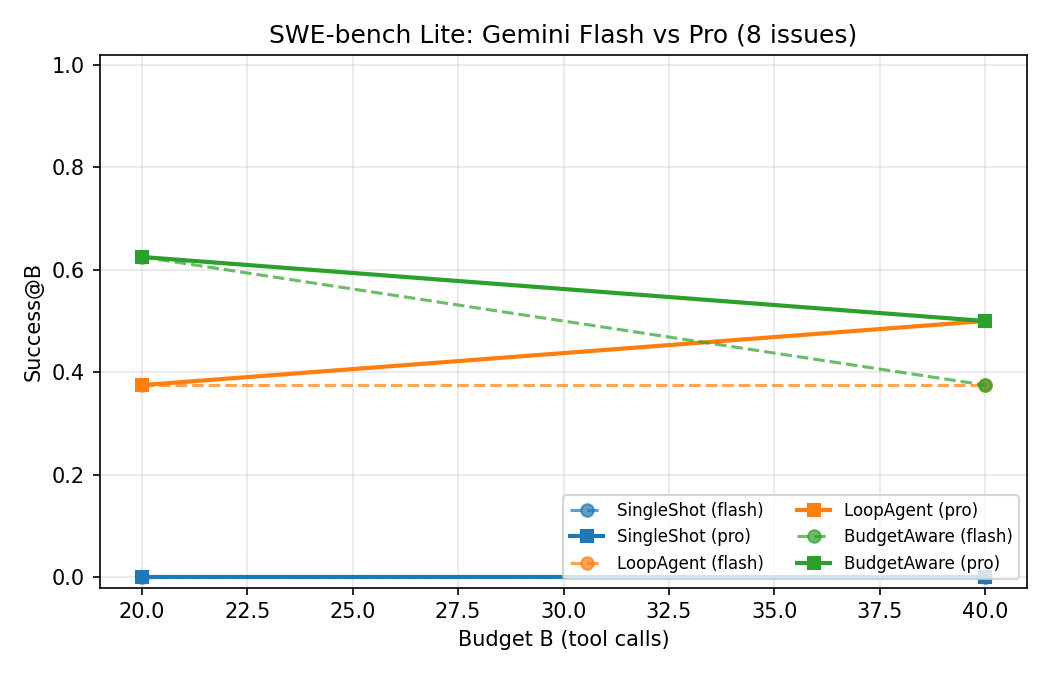
\includegraphics[width=0.85\textwidth]{swe_flash_vs_pro.png}
  \caption{SWE-bench Lite: Success@B for Flash (dashed) versus Pro
  (solid). Pro adds zero at $B = 20$ but $\sim$12 pp at $B = 40$ for
  the multi-step agents, suggesting Pro needs sufficient budget to
  use its capability. SingleShot remains at zero across both models
  and budgets.}
  \label{fig:swe-flash-pro}
\end{figure}

\begin{figure}[t]
  \centering
  \begin{subfigure}[b]{0.48\textwidth}
    \centering
    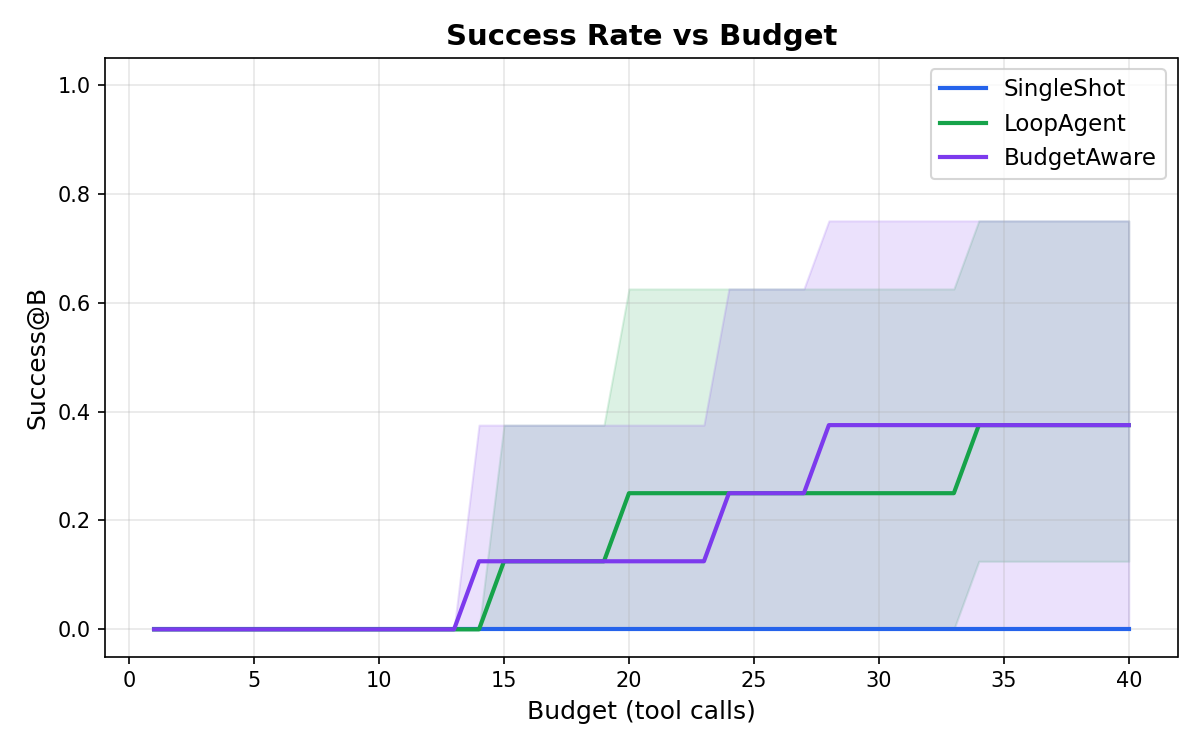
\includegraphics[width=\textwidth]{../results/swe_8issues_flash/success_curve.png}
    \caption{Success@B by agent.}
  \end{subfigure}
  \hfill
  \begin{subfigure}[b]{0.48\textwidth}
    \centering
    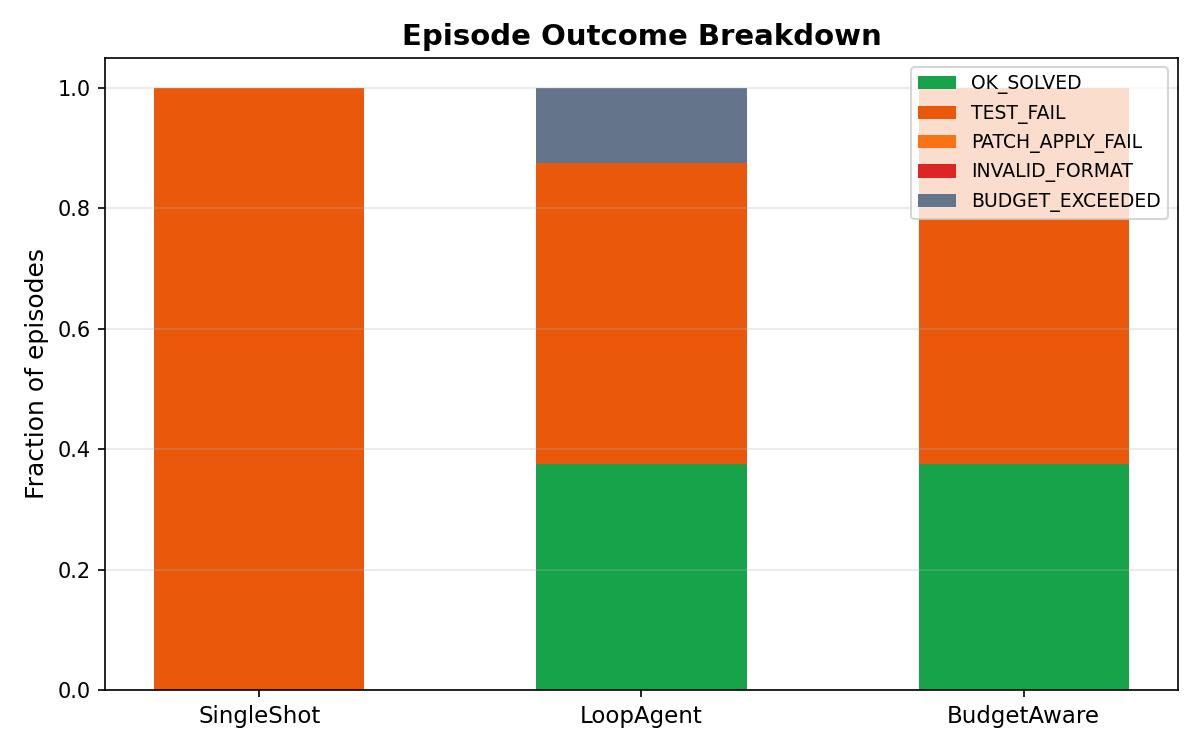
\includegraphics[width=\textwidth]{../results/swe_8issues_flash/status_bars.png}
    \caption{Episode status breakdown.}
  \end{subfigure}
  \caption{SWE-bench Lite (Gemini 2.5 Flash, 8 issues, 48 episodes
  total). BudgetAware peaks at $B = 20$ and never violates budget;
  LoopAgent ties on Success@40 but pays it back in budget exhaustion
  at $B = 20$.}
  \label{fig:swe}
\end{figure}

\subsection{Failure-Mode Analysis}
\label{sec:exp:failures}

Aggregating across both budgets, the failure-mode distribution
(Figure~\ref{fig:failures}) tells a clean story per agent. SingleShot
fails uniformly: 16 of 16 episodes terminate in \texttt{TEST\_FAIL},
i.e. the patch was syntactically valid but did not resolve the issue.
LoopAgent splits its failures roughly evenly between
\texttt{TEST\_FAIL} (37.5\%, six episodes) and
\texttt{BUDGET\_EXCEEDED} (25\%, four episodes). BudgetAware shows
no \texttt{BUDGET\_EXCEEDED} at all; its failures are entirely
\texttt{TEST\_FAIL} (50\%, eight episodes), which is the failure
mode we want, since these are recoverable with a better patch rather
than with more budget.

The hypothesis we set out to test was that LoopAgent's failure mix
would shift from \texttt{BUDGET\_EXCEEDED} at low budget to
\texttt{TEST\_FAIL} at high budget, indicating that more budget
trades violations for genuine attempts. Splitting LoopAgent's failures
by budget bears this out: at $B = 20$ three of five failures are
\texttt{BUDGET\_EXCEEDED}; at $B = 40$ only one of five is. The
remaining LoopAgent budget exceeds at $B = 40$ correspond to
particularly long astropy issues where even forty calls were not
enough exploration. We have no \texttt{INVALID\_FORMAT} failures in
this sample, an artifact of the explicit unified-diff format
enforcement in our patch-submission tool.

\begin{figure}[t]
  \centering
  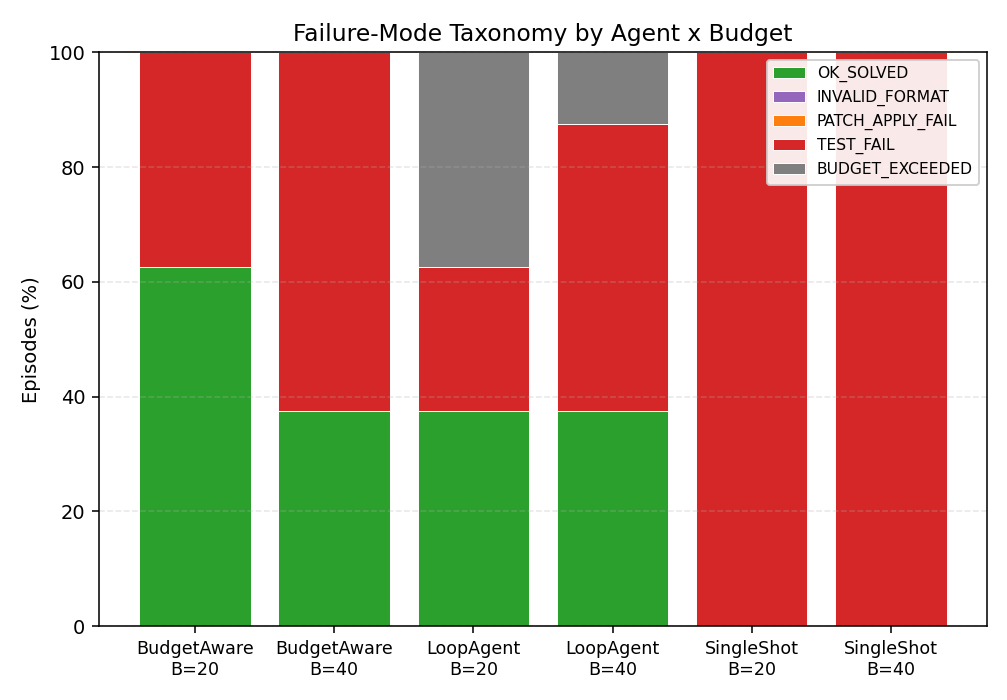
\includegraphics[width=0.85\textwidth]{../results/swe_8issues_flash/failures/failure_modes.png}
  \caption{SWE-bench Lite failure modes per agent (16 episodes per
  agent). SingleShot's failures are all \texttt{TEST\_FAIL};
  LoopAgent splits between \texttt{TEST\_FAIL} and
  \texttt{BUDGET\_EXCEEDED}; BudgetAware eliminates
  \texttt{BUDGET\_EXCEEDED} at the cost of one extra
  \texttt{TEST\_FAIL}.}
  \label{fig:failures}
\end{figure}

% -----------------------------------------------------------------------------
\section{Discussion}
\label{sec:discussion}

\paragraph{Strategy beats raw capability under budget.}
The most striking pattern in our data is the size gap between two
deltas. Switching from Flash to Pro adds about 8 percentage points of
success across all Knapsack cells, leaving the qualitative ordering
unchanged. Switching from LoopAgent to BudgetAwareAgent at $B = 10$
adds more than 50 percentage points (from $0$ to $0.62$ under Flash),
flipping the ordering completely. The first delta is the kind of
improvement a model upgrade gives you. The second is the kind of
improvement a strategy change gives you. In a budget-constrained
deployment, only the second is decisive.

\paragraph{The harness is cheap to add.}
The total BudgetBench surface area is small. The runner, metrics, and
visualisation modules together are roughly seven hundred lines of pure
Python with no LLM dependencies; an existing tool-using agent can opt
in by exposing its tool loop as the four-method
\texttt{Agent} interface, which in our experience requires under fifty
lines of glue per agent. The same runner could be retrofitted to
SWE-bench, ToolBench, or any other tool-using benchmark without
changing the underlying tasks, simply by treating the existing
benchmark as the Environment and capping the per-episode action count.

\paragraph{Design recommendations.}
Three concrete suggestions follow from our results for anyone building
a tool-using engineering agent that will operate under budget. First,
prefer an early-commit baseline. SingleShot is uncomfortably hard to
beat on AUC because it pays one unit and then nothing; agents that
explore must justify their exploration with measurable accuracy gains.
Second, expose the remaining budget to the agent and act on it. The
single intervention that flipped LoopAgent's behaviour was telling
the agent how much of its budget it had left and giving it a
fallback path; the cost was about a hundred lines of code. Third,
treat \texttt{run\_tests} as the dominant cost item. It is three
times more expensive than every other tool in our weighting and
typically far more in wall-clock; pruning it under tight budgets
(BudgetAware's MEDIUM regime) is a cheap way to extend reach.

\paragraph{AUC reveals what Success@$B_\text{max}$ hides.}
SingleShot and BudgetAware tie on terminal Success@$B$ in our
Knapsack experiments at every budget we test, because both ultimately
produce the same greedy solution. They do not tie on AUC. SingleShot
reaches $0.62$ success at $B \ge 1$ and stays flat, giving AUC@20 of
$0.589$ under Flash. BudgetAware spends roughly seven units of budget
on exploration in the HIGH regime before falling back, so its
sub-budget Success@$b$ at $b < 7$ is approximately zero, dragging
AUC@20 down to $0.388$. The two agents are equally accurate but
unequally efficient, and Success@$B_\text{max}$ alone cannot tell them
apart. AUC therefore distinguishes agents that reach their answer
quickly from agents that reach the same answer late, which is
precisely the gap that motivates budget-aware evaluation.

% -----------------------------------------------------------------------------
\section{Limitations}
\label{sec:limitations}

Our study has six limitations worth flagging.

\textit{(1) Small SWE-bench sample.} Eight issues drawn from the
default ordering of SWE-bench Lite are enough to surface the
qualitative ordering of agents but not enough to produce tight
confidence intervals on Success@$B$. Scaling to the full Lite split
(300 issues) would tighten the bands roughly six-fold and is the
single most useful follow-up.

\textit{(2) Tool-call budget, not token or wall-clock budget.}
Counting tool calls is a coarse proxy for the dollar and latency cost
that practitioners actually pay. A token-aware budget would handle the
case where one agent issues fewer but larger tool calls, and a
wall-clock budget would account for the dominance of \texttt{run\_tests}
in real test suites.

\textit{(3) Hand-tuned regime thresholds.} BudgetAware's $0.6$ and
$0.3$ thresholds were chosen by hand and held fixed across both
environments. Whether the same thresholds transfer to harder
benchmarks, or whether per-environment learned thresholds would help,
is open.

\textit{(4) Single LLM family.} We tested two Gemini 2.5 variants.
Replicating the Flash-versus-Pro story with a Claude or GPT family
backbone would test whether the eight-percentage-point ceiling on
model upgrades is universal or Gemini-specific.

\textit{(5) Heuristic Knapsack agents.} The Knapsack agents are
hand-coded heuristics rather than LLM-backed, which removes prompting
noise but also means the Knapsack results speak only to the harness,
not to LLM Knapsack skill. SWE-bench is the load-bearing experiment
for LLM-related claims.

\textit{(6) Retrieval augmentation deferred.} Our original proposal
included a lightweight retrieval-augmentation module over repository
context. We descoped this component to keep the budget-awareness
study a clean comparison; adding retrieval changes both the cost
profile and the action space and would have confounded the Flash-vs-Pro
and LoopAgent-vs-BudgetAware contrasts. The harness already supports
retrieval as a tool, and integrating it is a straightforward
follow-up.

% -----------------------------------------------------------------------------
\section{Conclusion}
\label{sec:conclusion}

Existing code-agent benchmarks score the answer and ignore the cost of
producing it. BudgetBench treats the tool-call budget as the central
axis: every action is intercepted, every cost is logged, and Success@B,
AUC, and the violation rate are reported with bootstrap intervals.
Across 900 Knapsack episodes and 96 SWE-bench Lite episodes, a
regime-switching BudgetAwareAgent matched or beat a single-shot
baseline's terminal accuracy with a zero violation rate while a
budget-blind ReAct loop collapsed at low budgets. Switching
the LLM backbone from Gemini Flash to Pro added a uniform 8 percentage
points but did not change the ordering. The harness is small,
LLM-agnostic, and could be retrofitted to existing benchmarks with a
thin shim, turning every tool-using-agent paper into one that also
reports its action efficiency.

% -----------------------------------------------------------------------------
\section*{Author Contributions}

\textbf{Chenrui Xu} designed and implemented the BudgetBench framework
(BudgetRunner, metrics, visualisation), the Knapsack environment, the
BudgetAwareAgent, the batch experiment harness, and led the writing of
this paper. \textbf{Hanyu Jin} implemented the SWE-bench environment
including the Docker sandbox and the harness-plus-fallback scoring
pipeline, the image-prebuild script, and contributed prompt-engineering
improvements to all three agents. \textbf{Sylvia Li} contributed to
agent-design discussions, prepared the presentation deck, and
delivered the in-class talk.

\section*{Code and Data Availability}

The full source, including the BudgetRunner, both environments, all three
agents, and the experiment scripts used to produce every figure and table
in this paper, is at \url{https://github.com/Eric-XC/budgetbench}. Raw
per-episode logs (CSV) are checked in under \texttt{results/}.

% -----------------------------------------------------------------------------
\bibliographystyle{plain}
\bibliography{refs}

\end{document}
